
The CWP is interpreted as LTL properties by breaking it into two sets: global and state properties. The global properties are:
\begin{enumerate}
    \item The system is always in one of the states
    \item The system eventually reaches one of the goal states
\end{enumerate}

State properties are generated for each state in the CWP, and ensure the following:
\begin{enumerate}
    \item The state is reachable in the system
    \item When the system is in a state, it is only in that state
    \item When the system moves from the current state, it only moves to a state that has a transition from the current state
\end{enumerate}

The CWP states are defined as boolean expressions using the edges as atomic propositions. The CWP is said to reside in a state when the following expression is true: 

\[(I_0 \land I_1 \land \ldots \land I_n) \land \neg (O_0 \ O_1 \lor \ldots \lor O_m)\]

where $I_0, I_1 \ldots I_n$ are incoming edges and $O_0, O_1 \ldots O_m$ are outgoing edges. The number of incoming edges is $n$ and the number of outgoing edges is $m$. 

\figref{fig:CWPStateDefinition} shows the CWP from the simple example given in the previous section with the edges labelled with letters from A to E. Using these labels, the definition of the \lstinline[style=myPromela]{Negotiations} state looks like this:

\begin{lstlisting}[style=myPromela]
Negotiations =
    (
        (EdgeA)
        &&
        (! (EdgeC || EdgeD))
    )
\end{lstlisting}

\begin{figure*}[t]
  \begin{center}
    \begin{tabular}{c}
        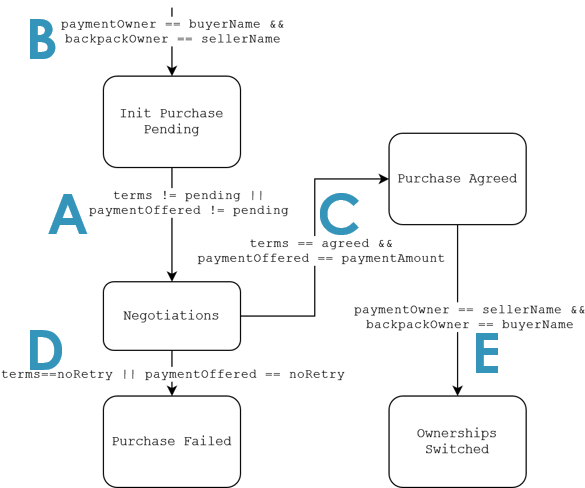
\includegraphics[width=\textwidth]{../figs/Other/CWPStateDefinition.png}
    \end{tabular}
  \end{center}
\caption{CWP for a purchase with the edges labelled}
\label{fig:CWPStateDefinition}
\end{figure*}

Once each of the states is property defined, we can begin to construct the LTL properties using these states as atomic propositions. The complete mathematical definition for each property will not be given in this paper, but an example with state property number two, or mutual exclusion, will be shown for the \lstinline[style=myPromela]{Negotiations} state in the purchase CWP.

\figref{fig:MutualExclusionExample} shows a visualization of the property, as it ensures that when a given state resolves to be true, all other states must resolve to be false. This is what the LTL property looks like for this example:

\begin{lstlisting}[style=myPromela]
ltl NegotiationsMutex {
    (
        always (
            Negotiations implies (
                Negotiations
                && (! Init_Purchase_Pending)
                && (! Purchase_Failed)
                && (! Ownerships_Switched)
                && (! Purchase_Agreed)
            )
        )
    )
}
\end{lstlisting}

\begin{figure*}[t]
  \begin{center}
    \begin{tabular}{c}
        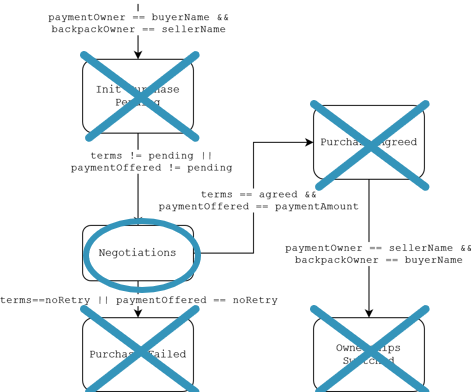
\includegraphics[width=\textwidth]{../figs/Other/MutualExclusionExample.png}
    \end{tabular}
  \end{center}
\caption{CWP for a purchase with annotations to assist in understanding the mutual exclusion property}
\label{fig:MutualExclusionExample}
\end{figure*}
